\newpage
\section{Visualizzazione profilo}
Dopo l'autenticazione, sarà possibile visualizzare i dati relativi al proprio profilo cliccando sulla prima voce del nuovo elenco presente sulla barra di sinistra:

\label{VaiProfilo}
\begin{figure}[ht]
	\centering
	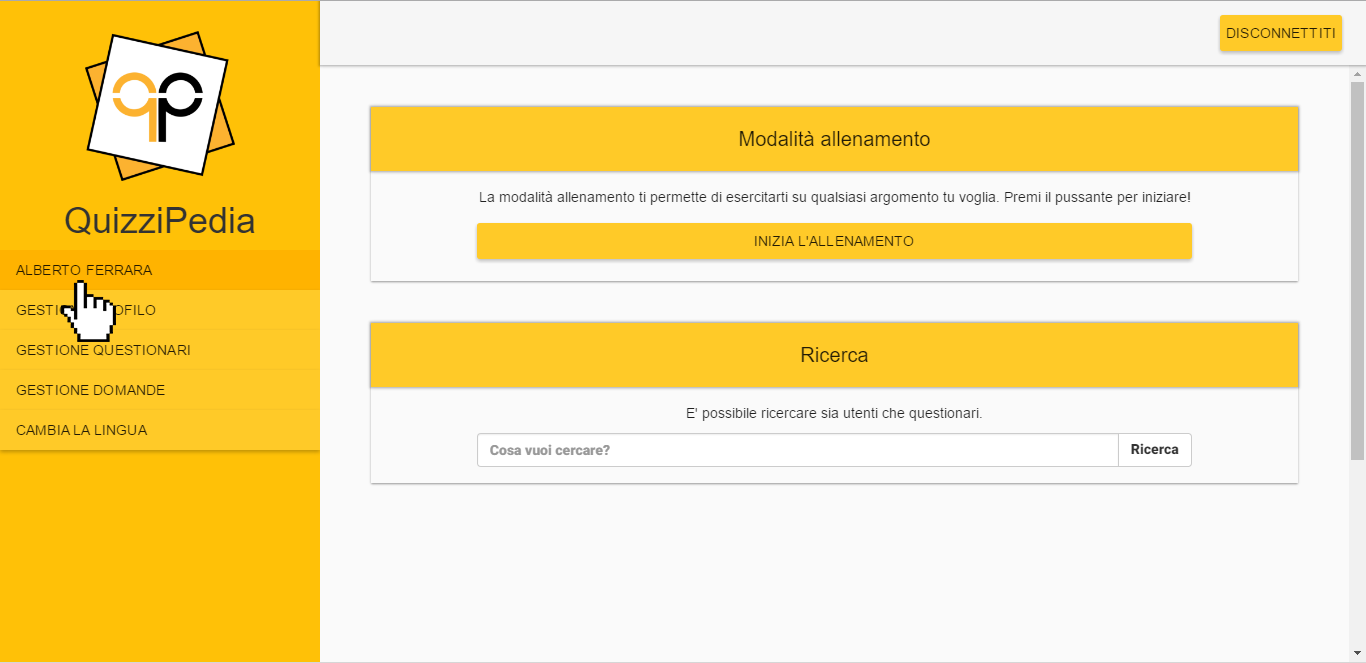
\includegraphics[scale=0.33]{img/vai_profilo.png}
	\caption{Vai a Visualizzazione profilo}
\end{figure}
\FloatBarrier

Verrà presentata una pagina contenente tutti i dati relativi al proprio profilo utente. In particolare sarà possibile visualizzare la cronologia dei questionari svolti:

\label{CronologiaQuestionari}
\begin{figure}[ht]
	\centering
	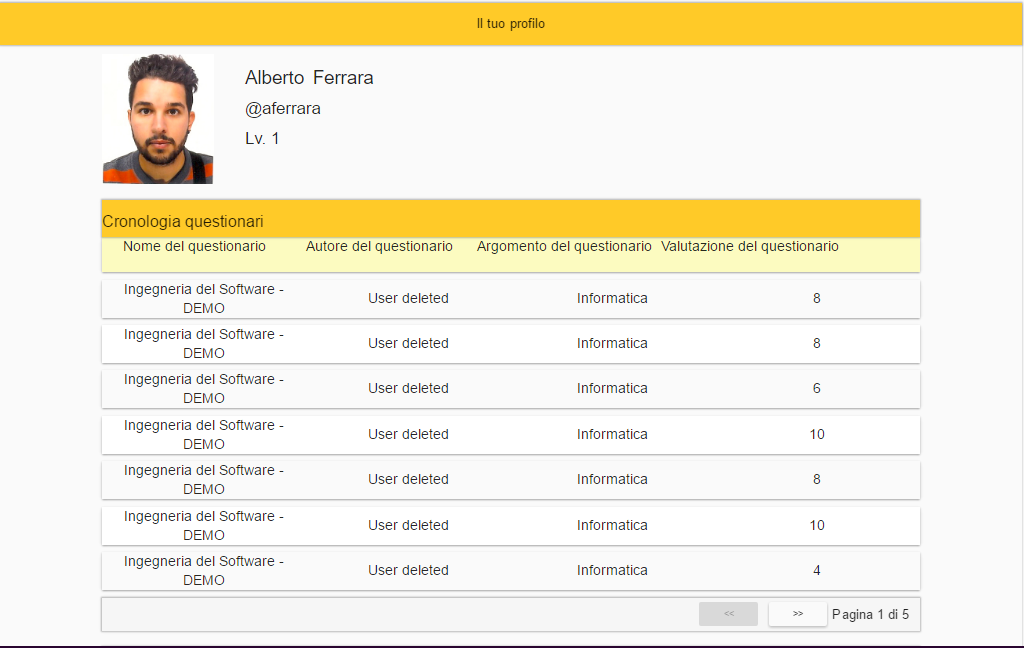
\includegraphics[scale=0.40]{img/cronologia_questionari.png}
	\caption{Cronologia questionari svolti}
\end{figure}
\FloatBarrier

i questionari a cui si è iscritti: 

\label{QuestionariIscritto}
\begin{figure}[ht]
	\centering
	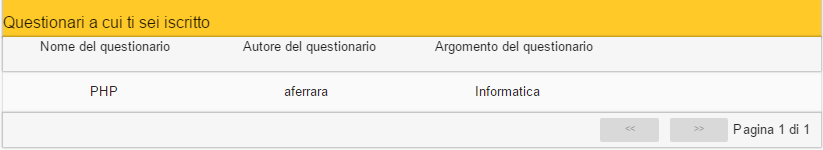
\includegraphics[scale=0.45]{img/questionari_iscritto.png}
	\caption{Questionari a cui si è iscritti}
\end{figure}
\FloatBarrier

e le proprie statistiche personali:

\label{StatistichePersonali}
\begin{figure}[ht]
	\centering
	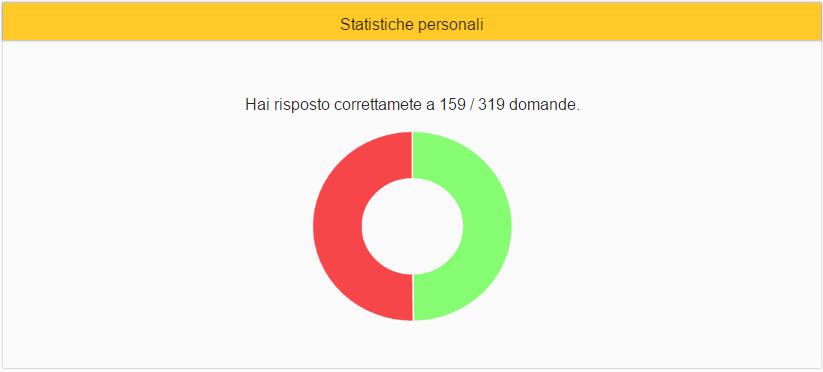
\includegraphics[scale=0.45]{img/statistiche_personali.png}
	\caption{Questionari a cui si è iscritti}
\end{figure}
\FloatBarrier